\documentclass{article}
\usepackage[utf8]{vietnam}
\usepackage{hyperref}
\hypersetup{
    colorlinks=true,
    linkcolor=blue,
    filecolor=magenta,      
    urlcolor=cyan,
}
\usepackage{parskip} % Package to tweak paragraph skipping
\setlength{\parskip}{1em}

\usepackage{amsmath}
\usepackage{amsfonts}
\usepackage{amssymb}
\usepackage{tikz,tkz-tab}

\title{Vẽ bảng biến thiên và bảng xét dấu}
\author{\textbf{Math2IT}\\ \href{http://math2it.com/huong-dan-ve-bang-bien-thien-va-bang-xet-dau-bang-goi-lenh-tkz-tab/}{math2it.com}}

\begin{document}
\maketitle


%===============================
Hàm số bậc nhất $y=ax+b$
\begin{center}
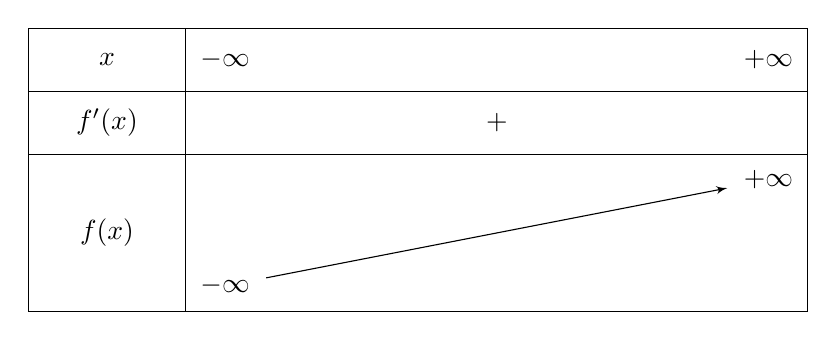
\begin{tikzpicture}
\tkzTabInit
[lgt=2,espcl=0.02\linewidth] % tùy chọn
{$x$/.8, $f’(x)$/.8, $f(x)$/2} % cột đầu tiên
{$-\infty$,$+\infty$} % hàng 1 cột 2
\tkzTabLine{,+,} % hàng 2 cột 2
\tkzTabVar{-/ $-\infty$ , +/ $+\infty$} % hàng 3 cột 2
\end{tikzpicture}
\end{center}


%===============================
Hàm số bậc hai $y=ax^2+bx+c$
\begin{center}
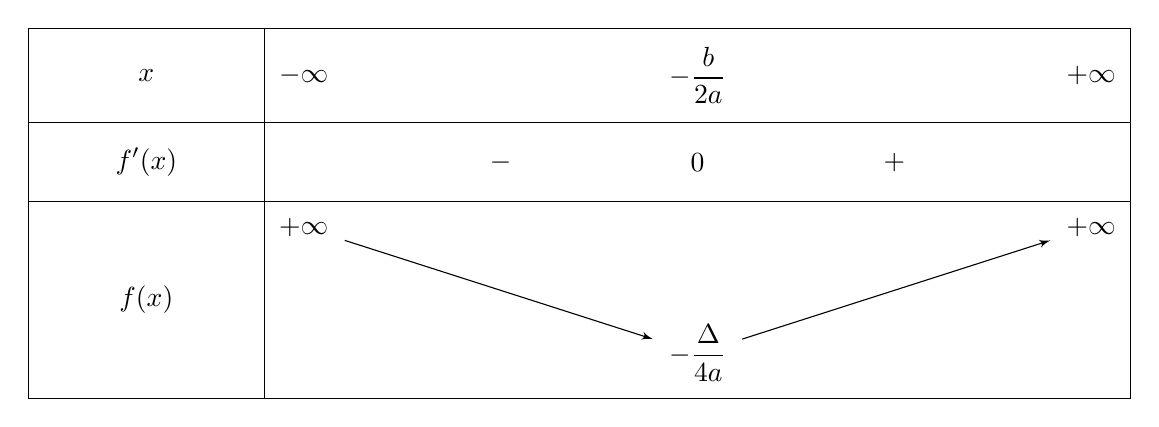
\begin{tikzpicture}
\tkzTabInit
[lgt=3,espcl=5] % tùy chọn
{$x$/1.2, $f’(x)$/1, $f(x)$/2.5} % cột đầu tiên
{$-\infty$, $-\dfrac{b}{2a}$, $+\infty$} % hàng 1 cột 2
\tkzTabLine{,-,0,+,} % hàng 2 cột 2
\tkzTabVar{+/ $+\infty$, -/ $-\dfrac{\Delta}{4a}$ , +/ $+\infty$} % hàng 3 cột 2
\end{tikzpicture}
\end{center}


%===============================
Hàm số bậc ba $y=ax^3+bx^2+cx+d$
\begin{center}
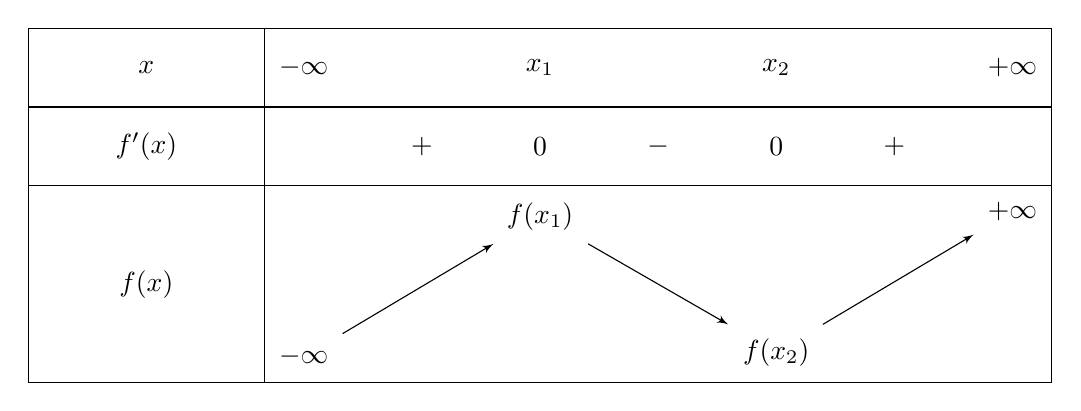
\begin{tikzpicture}
\tkzTab
[lgt=3,espcl=3] % tùy chọn
{$x$/1, $f’(x)$/1, $f(x)$/2.5} % cột đầu tiên
{$-\infty$, $x_1$, $x_2$, $+\infty$} % hàng 1 cột 2
{,+,0,-,0,+,} % hàng 2 cột 2
{-/ $-\infty$, +/ $f(x_1)$, -/ $f(x_2)$ , +/ $+\infty$} % hàng 3 cột 2
\end{tikzpicture}
\end{center}

\bigskip

\begin{center}
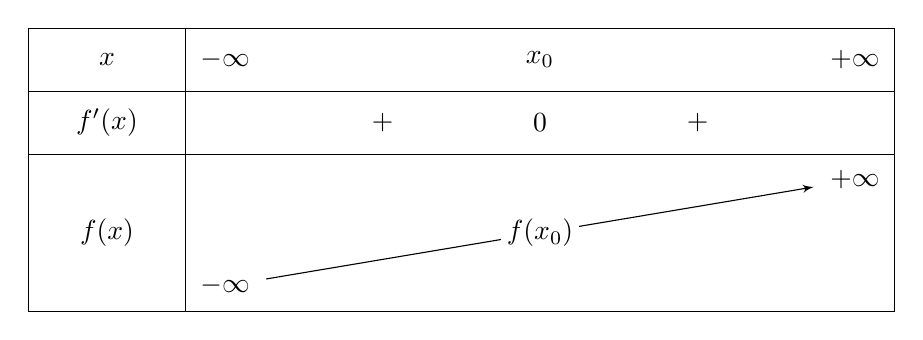
\begin{tikzpicture}
\tkzTabInit
[lgt=2,espcl=4] % tùy chọn
{$x$/0.8,$f’(x)$/0.8, $f(x)$/2} % cột đầu tiên
{$-\infty$,$x_0$,$+\infty$} % hàng 1 cột 2
\tkzTabLine{,+,0,+,} % hàng 2 cột 2
\tkzTabVar{-/ $-\infty$ , R/ , +/ $+\infty$} % hàng 3 cột 2 (2 điểm đầu)
\tkzTabIma{1}{3}{2}{$f(x_0)$} % hàng 3 cột 2 (điểm giữa)
\end{tikzpicture}
\end{center}


%===============================
Hàm số trùng phương $y=zx^4+bx^2+c$
\begin{center}
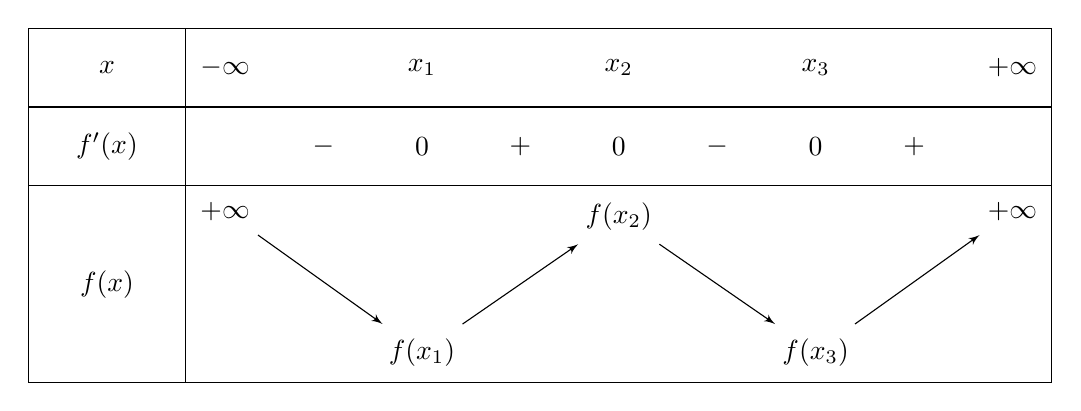
\begin{tikzpicture}
\tkzTab
[lgt=2,espcl=2.5] % tùy chọn
{$x$/1, $f’(x)$/1, $f(x)$/2.5} % cột đầu tiên
{$-\infty$, $x_1$, $x_2$, $x_3$, $+\infty$} % hàng 1 cột 2
{,-,0,+,0,-,0,+,} % hàng 2 cột 2
{+/ $+\infty$, -/ $f(x_1)$, +/ $f(x_2)$, -/ $f(x_3)$ , +/ $+\infty$} % hàng 3 cột 2
\end{tikzpicture}
\end{center}


%===============================
Hàm phân thức bậc nhất $y=\dfrac{ax+b}{cx+d}$
\begin{center}
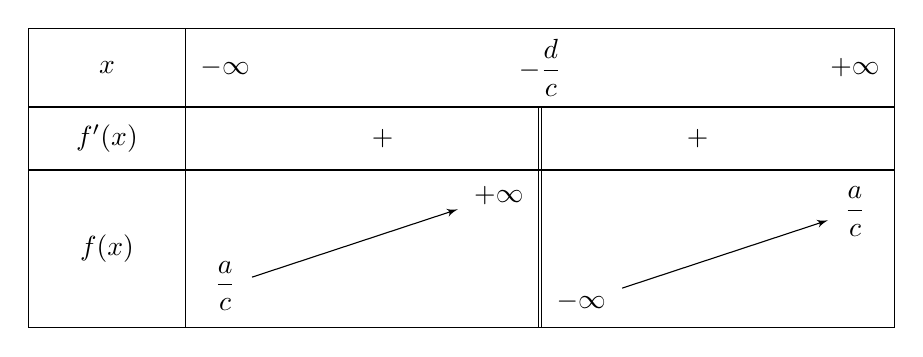
\begin{tikzpicture}
\tkzTab
[lgt=2,espcl=4] % tùy chọn
{$x$/1, $f’(x)$/0.8, $f(x)$/2} % cột đầu tiên
{$-\infty$, $-\dfrac{d}{c}$, $+\infty$} % hàng 1 cột 2
{,+,d,+,} % hàng 2 cột 2
{-/ $\dfrac{a}{c}$, +D-/ $+\infty$ / $-\infty$, +/ $\dfrac{a}{c}$} % hàng 3 cột 2
\end{tikzpicture}
\end{center}


%===============================
Hàm phân thức bậc hai $y=\dfrac{ax^2+bx+c}{dx+e}$
\begin{center}
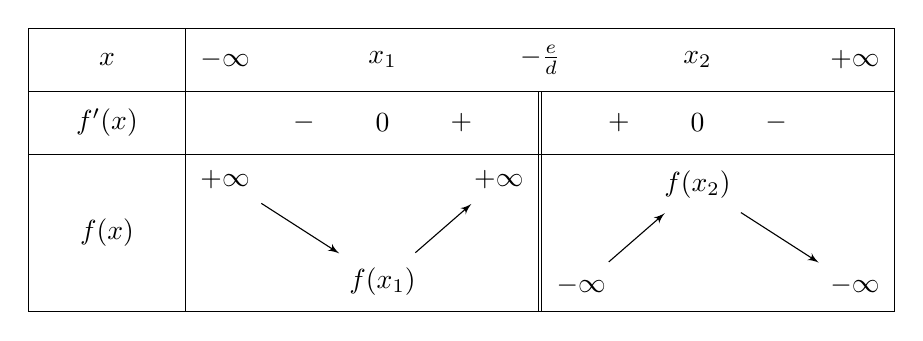
\begin{tikzpicture}
\tkzTab
[lgt=2,espcl=2] % tùy chọn
{$x$/0.8, $f’(x)$/0.8, $f(x)$/2} % cột đầu tiên
{$-\infty$, $x_1$, $-\frac{e}{d}$, $x_2$, $+\infty$} % hàng 1 cột 2
{,-,0,+,d,+,0,-,} % hàng 2 cột 2
{+/ $+\infty$, -/ $f(x_1)$, +D-/ $+\infty$ / $-\infty$, +/ $f(x_2)$, -/ $-\infty$} % hàng 3 cột 2
\end{tikzpicture}
\end{center}


%===============================
Bảng xét dấu
\begin{center}
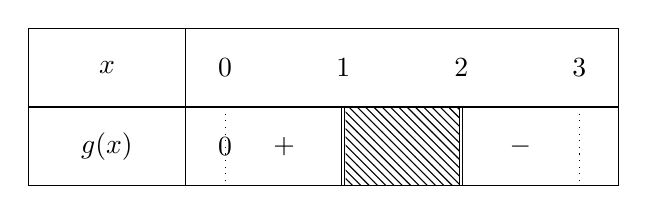
\begin{tikzpicture}
\tkzTabInit
[lgt=2,espcl=1.5] % tùy chọn
{$x$/1, $g(x)$/1} % cột 1
{$0$,$1$,$2$,$3$} % hàng 1 cột 2
\tkzTabLine{z, + , d , h , d , - , t} % hàng 2 cột 2
\end{tikzpicture}
\end{center}


%===============================
Thêm gạch sọc
\begin{center}
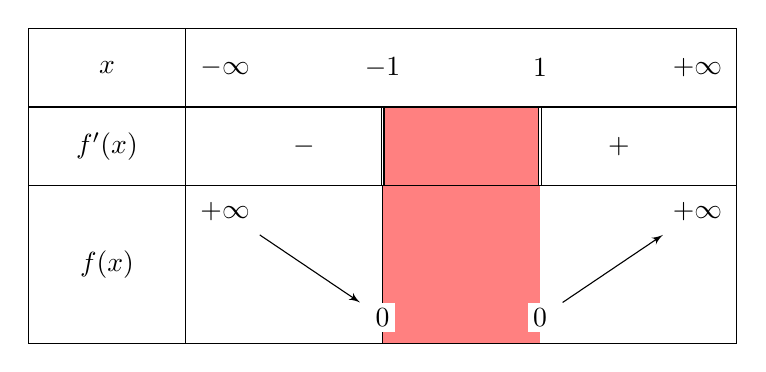
\begin{tikzpicture}
\tikzset{h style/.style = {fill=red!50}}
\tkzTab
[lgt=2,espcl=2] % tùy chọn
{$x$/1, $f’(x)$/1, $f(x)$/2} % cột đầu tiên
{ $-\infty$, $-1$, $1$, $+\infty$} % hàng 1 cột 2
{ ,-,d,h,d,+, } % hàng 2 cột 2
{ +/$+\infty$ , -H/$0$, -/$0$ , +/ $+\infty$ } % hàng 3 cột 2
\end{tikzpicture}
\end{center}


%===============================
Tô màu thay cho gạch sọc
\begin{center}
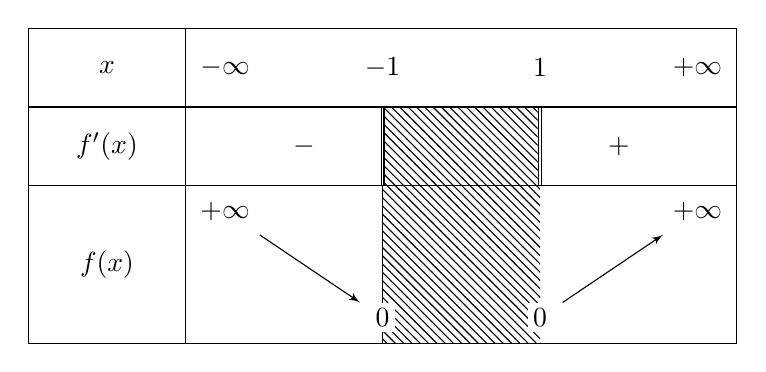
\begin{tikzpicture}
\tkzTab
[lgt=2,espcl=2] % tùy chọn
{$x$/1, $f’(x)$/1, $f(x)$/2} % cột đầu tiên
{ $-\infty$, $-1$, $1$, $+\infty$} % hàng 1 cột 2
{ ,-,d,h,d,+, } % hàng 2 cột 2
{ +/$+\infty$ , -H/$0$, -/$0$ , +/ $+\infty$ } % hàng 3 cột 2
\end{tikzpicture}
\end{center}



%===============================
Gạch chéo xóa bảng
\begin{center}
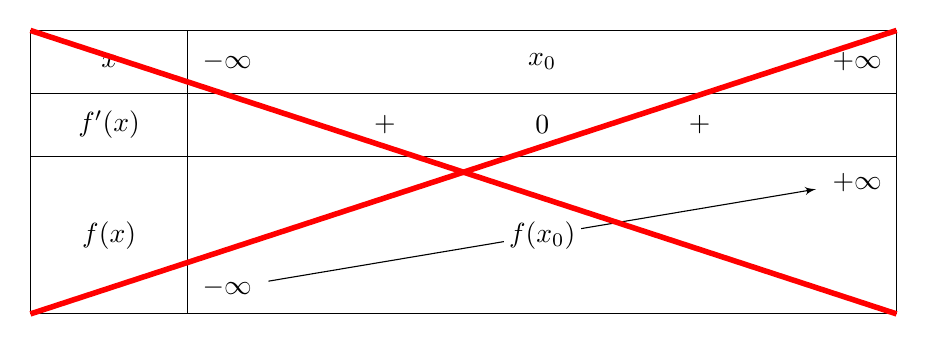
\begin{tikzpicture}
\tkzTabInit
[lgt=2,espcl=4] % tùy chọn
{$x$/0.8,$f’(x)$/0.8, $f(x)$/2} % cột đầu tiên
{$-\infty$,$x_0$,$+\infty$} % hàng 1 cột 2
\tkzTabLine{,+,0,+,} % hàng 2 cột 2
\tkzTabVar{-/ $-\infty$ , R/ , +/ $+\infty$} % hàng 3 cột 2 (2 điểm đầu)
\tkzTabIma{1}{3}{2}{$f(x_0)$} % hàng 3 cột 2 (điểm giữa)
\draw[line width=2pt,red] (T00) to (T23);
\draw[line width=2pt,red] (T03) to (T20);
\end{tikzpicture}
\end{center}


%===============================
Gạch chéo xóa 1 phần bảng
\begin{center}
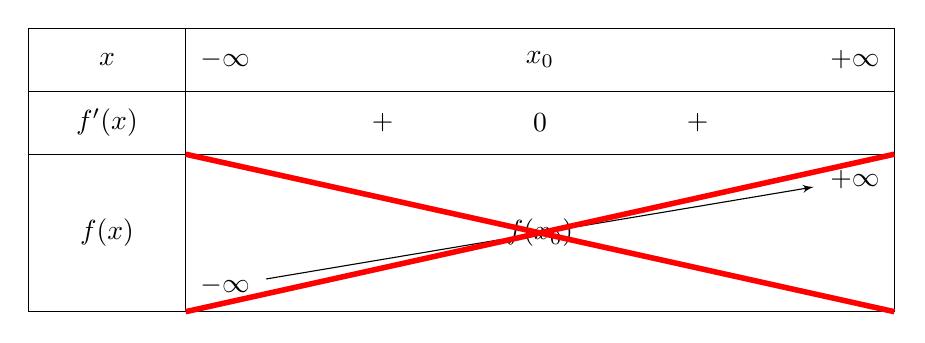
\begin{tikzpicture}
\tkzTabInit
[lgt=2,espcl=4] % tùy chọn
{$x$/0.8,$f’(x)$/0.8, $f(x)$/2} % cột đầu tiên
{$-\infty$,$x_0$,$+\infty$} % hàng 1 cột 2
\tkzTabLine{,+,0,+,} % hàng 2 cột 2
\tkzTabVar{-/ $-\infty$ , R/ , +/ $+\infty$} % hàng 3 cột 2 (2 điểm đầu)
\tkzTabIma{1}{3}{2}{$f(x_0)$} % hàng 3 cột 2 (điểm giữa)
\draw[line width=2pt,red] (T12) to (T23);
\draw[line width=2pt,red] (T13) to (T22);
\end{tikzpicture}
\end{center}


%===============================
Mất viền khung ngoài cùng
\begin{center}
\begin{tikzpicture}
\tkzTabInit
[lgt=2,espcl=4,nocadre] % tùy chọn
{$x$/0.8,$f’(x)$/0.8, $f(x)$/2} % cột đầu tiên
{$-\infty$,$x_0$,$+\infty$} % hàng 1 cột 2
\tkzTabLine{,+,0,+,} % hàng 2 cột 2
\tkzTabVar{-/ $-\infty$ , R/ , +/ $+\infty$} % hàng 3 cột 2 (2 điểm đầu)
\tkzTabIma{1}{3}{2}{$f(x_0)$} % hàng 3 cột 2 (điểm giữa)
\end{tikzpicture}
\end{center}


Tô màu cho các ô
\begin{center}
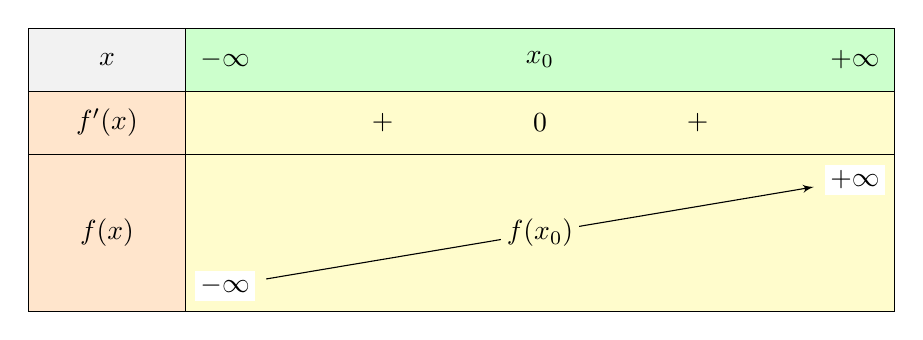
\begin{tikzpicture}
\tkzTabInit
[lgt=2,espcl=4, % độ rộng
nocadre, % làm mất viền
color, % tô màu
colorT = yellow!20, % phần chính của bảng
colorC = orange!20, % cột đầu
colorL = green!20, % hàng đầu
colorV = lightgray!20 % biến
] % tùy chọn
{$x$/0.8,$f’(x)$/0.8, $f(x)$/2} % cột đầu tiên
{$-\infty$,$x_0$,$+\infty$} % hàng 1 cột 2
\tkzTabLine{,+,0,+,} % hàng 2 cột 2
\tkzTabVar{-/ $-\infty$ , R/ , +/ $+\infty$} % hàng 3 cột 2 (2 điểm đầu)
\tkzTabIma{1}{3}{2}{$f(x_0)$} % hàng 3 cột 2 (điểm giữa)
\end{tikzpicture}
\end{center}


\end{document}